%%
%% LoopGym: Invariants without Targets — Learning Inductive Loop Summaries
%%          with Execution-Grounded, Audited Rewards
%% NeurIPS 2024 Format
%%
\documentclass[11pt]{article}

%% NeurIPS style
\usepackage[preprint]{neurips_2024}

%% Packages
\usepackage{booktabs}
\usepackage{listings}
\usepackage{xcolor}
\usepackage{subcaption}
\usepackage{amsmath}
\usepackage{amssymb}
\usepackage{pifont}
\usepackage{amsthm}
\usepackage{graphicx}
\usepackage{hyperref}
\usepackage{url}
\usepackage{microtype}
\usepackage{tcolorbox}
\usepackage{enumitem}
\usepackage{multirow}
\usepackage{natbib}
\usepackage{float}
\usepackage{tikz}
\usetikzlibrary{calc,arrows.meta,positioning}

%% tcolorbox setup
\tcbuselibrary{skins,breakable}

%% Theorem environments
\newtheorem{theorem}{Theorem}
\newtheorem{proposition}[theorem]{Proposition}
\newtheorem{definition}[theorem]{Definition}

%% ---- Custom algorithm environment (NeurIPS-style) ----
\newfloat{algorithm}{tbp}{loa}
\floatname{algorithm}{Algorithm}

\newcounter{alglinenum}
\newenvironment{algorithmic}{%
  \setcounter{alglinenum}{0}%
  \par\small\noindent
  \begin{tabbing}%
  \hspace{1.8em}\=\hspace{1.2em}\=\kill
}{%
  \end{tabbing}%
}
\newcommand{\algline}{\stepcounter{alglinenum}{\scriptsize\makebox[1.8em][r]{\arabic{alglinenum}:\;}}\>}
\newcommand{\algind}{\>}
\newcommand{\kw}[1]{\textbf{#1}}
\newcommand{\cmnt}[1]{\hfill{\color{codegray}\itshape$\triangleright$ #1}}
\newcommand{\alginput}[1]{\hspace{1.8em}\textbf{Input:} #1\\}
\newcommand{\algoutput}[1]{\hspace{1.8em}\textbf{Output:} #1\\}
\newcommand{\algblank}{\\[-4pt]}

%% Colors
\definecolor{codeblue}{HTML}{2563EB}
\definecolor{codegray}{HTML}{6B7280}
\definecolor{codepurple}{HTML}{7C3AED}
\definecolor{codered}{HTML}{DC2626}
\definecolor{codegreen}{HTML}{059669}
\definecolor{promptbg}{HTML}{F8FAFC}
\definecolor{promptframe}{HTML}{CBD5E1}
\definecolor{algobg}{HTML}{F0F9FF}
\definecolor{algoframe}{HTML}{93C5FD}

%% Listings style for C / ACSL
\lstdefinestyle{cstyle}{
  language=C,
  basicstyle=\ttfamily\small,
  keywordstyle=\color{codeblue}\bfseries,
  commentstyle=\color{codegray}\itshape,
  stringstyle=\color{codered},
  numbers=left,
  numberstyle=\tiny\color{codegray},
  stepnumber=1,
  numbersep=6pt,
  backgroundcolor=\color{white},
  showspaces=false,
  showstringspaces=false,
  showtabs=false,
  frame=l,
  rulecolor=\color{codeblue!40},
  framesep=4pt,
  framerule=2pt,
  tabsize=2,
  captionpos=b,
  breaklines=true,
  breakatwhitespace=false,
  escapeinside={(*@}{@*)},
  morekeywords={loop,invariant,assigns,variant,requires,assert},
  literate={\\at}{{{\color{codeblue}\textbackslash at}}}3
           {\\forall}{{{\color{codeblue}\textbackslash forall}}}7
           {\\exists}{{{\color{codeblue}\textbackslash exists}}}7,
  aboveskip=0.8em,
  belowskip=0.5em,
}
\lstset{style=cstyle}

%% Listings style for prompts
\lstdefinestyle{promptstyle}{
  language=,
  basicstyle=\ttfamily\scriptsize,
  keywordstyle=\color{codeblue}\bfseries,
  commentstyle=\color{codegray}\itshape,
  numbers=none,
  frame=none,
  breaklines=true,
  columns=fullflexible,
  keepspaces=true,
  morekeywords={},
  aboveskip=0pt,
  belowskip=0pt,
}

%% Prompt box environment
\newtcolorbox{promptbox}[1][]{
  enhanced,
  breakable,
  colback=promptbg,
  colframe=promptframe,
  boxrule=0.5pt,
  arc=3pt,
  left=6pt,
  right=6pt,
  top=5pt,
  bottom=5pt,
  fonttitle=\small\bfseries\sffamily,
  title={#1},
  coltitle=black,
  colbacktitle=promptframe!30,
  attach boxed title to top left={yshift=-2mm,xshift=4mm},
  boxed title style={arc=2pt,boxrule=0pt},
}

%% Pipeline step box
\newtcolorbox{stepbox}[1][]{
  enhanced,
  colback=white,
  colframe=codeblue!60,
  boxrule=0.6pt,
  arc=2pt,
  left=5pt,
  right=5pt,
  top=4pt,
  bottom=4pt,
  fontupper=\small,
  title={#1},
  fonttitle=\small\bfseries\sffamily,
  coltitle=white,
  colbacktitle=codeblue!70,
  attach boxed title to top left={yshift=-2mm,xshift=4mm},
  boxed title style={arc=2pt,boxrule=0pt},
}

%% Shorthand commands
\newcommand{\cmark}{\ding{51}}
\newcommand{\xmark}{\ding{55}}
\newcommand{\sam}{\textsc{LoopGym}}

%% Meta
\title{Invariants without Targets: Learning Inductive Loop Summaries\\with Execution-Grounded, Audited Rewards}

\author{
  Anonymous Author(s)\\
  Anonymous Institution\\
  \texttt{anonymous@example.com}
}

\begin{document}

\maketitle

\begin{abstract}
Loop invariant generation is a central challenge in program verification, and four decades of work---abstract interpretation, constraint solving, data-driven learning, and most recently large language models---have framed it almost uniformly as a \emph{target-directed} task: given a program \emph{and a verification target} (a postcondition or assertion), find an inductive invariant strong enough to discharge the target.
We argue that this framing rests on a circularity that limits practical impact: verification targets are scarce in real code, writing them is itself the specification bottleneck, and for loop programs the target is typically nothing but the projection of an invariant at loop exit ($I \wedge \neg B \Rightarrow Q$)---whoever wrote $Q$ had already done the invariant reasoning.
We therefore reframe the task as generating an \emph{inductive loop summary}: the strongest practically expressible inductive invariant that characterizes a loop's reachable states, synthesized \emph{closed-book}, with no postcondition visible to the generator.
Removing the target removes the binary verifier signal that prior learning approaches optimize, so we develop an execution-grounded dense reward suitable for reinforcement learning.  Its sampler constructs three families of synthetic negative candidates---dense-neighborhood relational perturbations, genuine-exit over-run continuations, and sampled-range escapes---and conservatively suppresses candidates contradicted by sampled reachability, fresh-entry feasibility, or incomplete state/control coverage.
Candidate invariants are reduced by an always-on cascade ending in Houdini-style Frama-C/WP pruning.  For each rollout, the complete generation reward is an equal-weighted sum of its standalone negative rejection rate and its marginal contribution to the group union, with no auxiliary scoring terms.
The result, \sam{}, is an open three-component pipeline---sampler, reward service, and inference framework.  The current discrimination regression covers 10 deterministic programs, while a full-suite audit compared 486,302 sampled negative witnesses across 366 linear and nonlinear programs with larger reachable-state samples and found zero hard mislabels.
\end{abstract}

%% ============================================================
%% ============================================================
\section{Introduction}\label{sec:intro}
%% ============================================================

%% ============================================================
%% Figure 1: main overview figure
%% ============================================================
\begin{figure}[t]
\centering
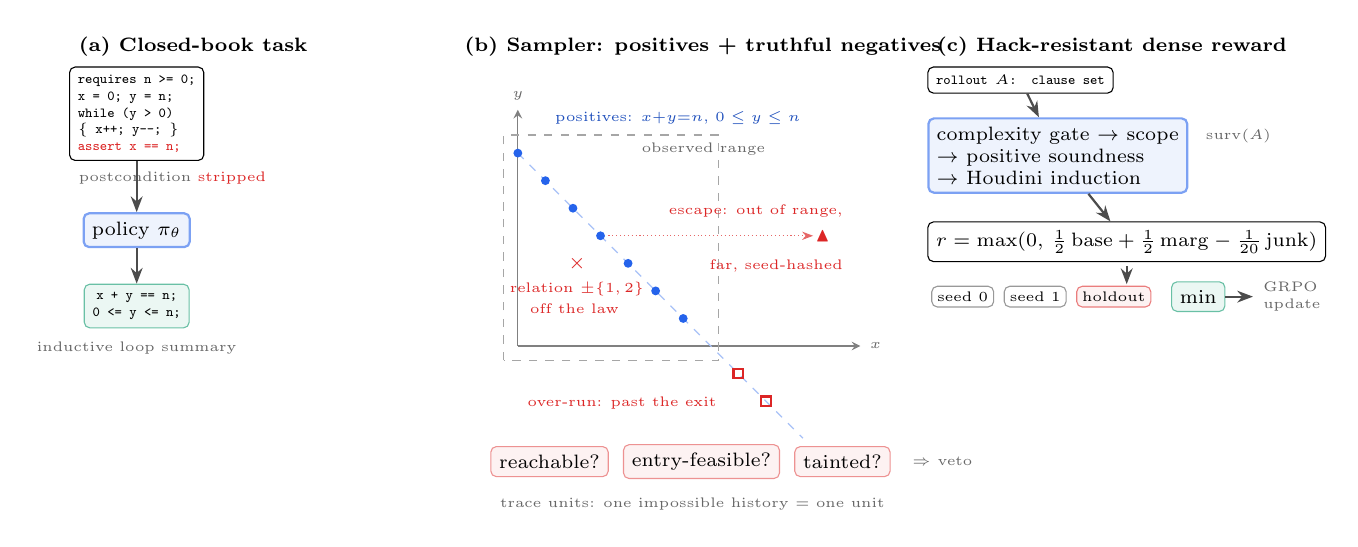
\begin{tikzpicture}[
  font=\scriptsize,
  box/.style={draw, rounded corners=2pt, align=center, inner sep=3pt},
  stage/.style={box, fill=codeblue!8, draw=codeblue!60, thick},
  neg/.style={box, fill=codered!6, draw=codered!50},
  chip/.style={box, fill=white, draw=black!40, inner sep=2pt, font=\tiny},
  arr/.style={-{Stealth[length=2mm]}, thick, black!70},
  lbl/.style={font=\tiny, black!60},
  >=stealth,
]
%% ---------------- panel (a): task ----------------
\node[anchor=north west] (atitle) at (0,5.6) {\textbf{(a) Closed-book task}};
\node[box, anchor=north west, fill=white, font=\ttfamily\tiny, align=left]
  (prog) at (0,5.1) {
    requires n >= 0;\\
    x = 0; y = n;\\
    while (y > 0)\\
    \{ x++; y--; \}\\
    \textcolor{codered}{\sout{assert x == n;}}
  };
\node[lbl, anchor=west] at ($(prog.south west)+(0,-0.22)$) {postcondition \textcolor{codered}{stripped}};
\node[stage, anchor=north] (pol) at ($(prog.south)+(0,-0.65)$) {policy $\pi_\theta$};
\node[box, anchor=north, fill=codegreen!8, draw=codegreen!60, font=\ttfamily\tiny]
  (summ) at ($(pol.south)+(0,-0.45)$) {x + y == n;\\ 0 <= y <= n;};
\node[lbl, anchor=north] at ($(summ.south)+(0,-0.05)$) {inductive loop summary};
\draw[arr] (prog) -- (pol);
\draw[arr] (pol) -- (summ);

%% ---------------- panel (b): sampler ----------------
\node[anchor=north west] (btitle) at (4.9,5.6) {\textbf{(b) Sampler: positives + truthful negatives}};
\begin{scope}[shift={(5.7,1.55)}]
  % axes
  \draw[->, black!50] (0,0) -- (4.35,0) node[right, lbl] {$x$};
  \draw[->, black!50] (0,0) -- (0,3.0) node[above, lbl] {$y$};
  % observed range box
  \draw[dashed, black!35] (-0.18,-0.18) rectangle (2.55,2.68);
  \node[lbl, anchor=west] at (1.45,2.5) {observed range};
  % manifold x+y=n, extended past the exit
  \draw[codeblue!40, dashed] (0,2.45) -- (3.62,-1.17);
  % positives on the manifold
  \foreach \i in {0,...,6} {
    \fill[codeblue] ({0.35*\i},{2.45-0.35*\i}) circle (1.6pt);
  }
  \node[lbl, text=codeblue!80!black, anchor=west] at (0.35,2.9) {positives: $x{+}y{=}n$, $0 \le y \le n$};
  % relation negative: off the manifold
  \node[text=codered] at (0.75,1.05) {$\times$};
  \node[lbl, text=codered] at (0.75,0.72) {relation $\pm\{1,2\}$};
  \node[lbl, text=codered] at (0.72,0.47) {off the law};
  % escape: push one variable out of range, dotted displacement arrow
  \draw[densely dotted, codered!70, -{Stealth[length=1.4mm]}] (1.15,1.4) -- (3.75,1.4);
  \node[text=codered] at (3.87,1.4) {$\blacktriangle$};
  \node[lbl, text=codered, anchor=east] at (4.25,1.72) {escape: out of range,};
  \node[lbl, text=codered, anchor=east] at (4.25,1.02) {far, seed-hashed};
  % over-run continuation: on the manifold, past the exit
  \foreach \i in {8,9} {
    \draw[codered, thick] ({0.35*\i-0.06},{2.45-0.35*\i-0.06}) rectangle ({0.35*\i+0.06},{2.45-0.35*\i+0.06});
  }
  \node[lbl, text=codered, anchor=west] at (0.0,-0.72) {over-run: past the exit};
\end{scope}
% filter strip
\node[neg, anchor=north west] (f1) at (5.35,0.28) {reachable?};
\node[neg, anchor=west] (f2) at ($(f1.east)+(0.18,0)$) {entry-feasible?};
\node[neg, anchor=west] (f3) at ($(f2.east)+(0.18,0)$) {tainted?};
\node[lbl, anchor=west] at ($(f3.east)+(0.15,0)$) {$\Rightarrow$ veto};
\node[lbl, anchor=north west] at (5.35,-0.25) {trace units: one impossible history $=$ one unit};

%% ---------------- panel (c): reward ----------------
\node[anchor=north west] (ctitle) at (10.9,5.6) {\textbf{(c) Hack-resistant dense reward}};
\node[box, anchor=north west, font=\ttfamily\tiny, align=left] (roll) at (10.9,5.1)
  {rollout $A$: clause set};
\node[stage, anchor=north west, align=left] (casc) at ($(roll.south west)+(0,-0.3)$)
  {complexity gate $\to$ scope\\ $\to$ positive soundness\\ $\to$ Houdini induction};
\node[lbl, anchor=west] at ($(casc.east)+(0.1,0.25)$) {$\mathrm{surv}(A)$};
\node[box, anchor=north west, fill=white] (score) at ($(casc.south west)+(0,-0.35)$)
  {$r = \max(0,\, \tfrac12\,\mathrm{base} + \tfrac12\,\mathrm{marg} - \tfrac1{20}\,\mathrm{junk})$};
\node[chip, anchor=north west] (s0) at ($(score.south west)+(0.05,-0.3)$) {seed 0};
\node[chip, anchor=west] (s1) at ($(s0.east)+(0.12,0)$) {seed 1};
\node[chip, anchor=west, draw=codered!60, fill=codered!6] (sh) at ($(s1.east)+(0.12,0)$) {holdout};
\node[box, anchor=west, fill=codegreen!8, draw=codegreen!60] (min) at ($(sh.east)+(0.25,0)$) {$\min$};
\draw[arr] (roll) -- (casc);
\draw[arr] (casc) -- (score);
\draw[arr] ($(score.south)+(0,-0.05)$) -- ($(score.south)+(0,-0.28)$);
\draw[arr] (min.east) -- ++(0.35,0) node[anchor=west, lbl, align=left] {GRPO\\ update};
\end{tikzpicture}
\caption{\textbf{\sam{} overview.}
(a)~The policy sees only precondition, guard, and body---the postcondition is stripped---and must emit the \emph{strongest} inductive loop summary, not an invariant tailored to a given target.
(b)~The sampler executes the instrumented loop over a deterministic, precondition-respecting input sweep; positives are observed loop-head states, and negatives are \emph{truthful impossible traces} in two dimensions: relational perturbations off densely sampled trace windows, and bound violations (over-run continuations past a genuine exit, and seed-hashed range escapes).
Three vetoes (reachability, entry feasibility, nondeterminism taint) guarantee every emitted negative is unreachable under its input.
(c)~Each rollout is reduced to its surviving inductive core, scored by the fraction of impossible traces it rejects (plus ablation-based marginal credit and a junk discount), and \emph{minimized} across canonical and held-out sampling seeds, so memorizing any finite sample earns nothing.}
\label{fig:overview}
\end{figure}


Loop invariants are the linchpin of deductive program verification.
Ever since the inductive-assertion method of Floyd~\citep{floyd1967assigning} and the axiomatic semantics of Hoare~\citep{hoare1969axiomatic}, verifying a loop $\mathtt{while}\,(B)\,S$ against a contract $\{P\}\cdot\{Q\}$ has reduced to exhibiting an \emph{inductive invariant} $I$ satisfying initiation ($P \Rightarrow I$), consecution ($\{I \wedge B\}\,S\,\{I\}$), and safety ($I \wedge \neg B \Rightarrow Q$).
Finding $I$ automatically has consequently been one of the most intensively studied problems in formal methods.
Four decades of research have attacked it with abstract interpretation~\citep{cousot1977abstract,cousot1978automatic,karr1976affine}, constraint- and template-based synthesis~\citep{colon2003linear,sankaranarayanan2004non,gulwani2008program,gupta2009invgen}, interpolation and IC3/PDR-style generalization~\citep{mcmillan2003interpolation,bradley2011sat,komuravelli2014smt}, abductive inference~\citep{dillig2013inductive}, syntax-guided and stochastic search~\citep{alur2013sygus,fedyukovich2018syntax}, data-driven learning from program states~\citep{sharma2012interpolants,sharma2013data,garg2014ice,garg2016learning,padhi2016pie,zhu2018data,ezudheen2018horn}, neural architectures~\citep{si2018learning,si2020code2inv,ryan2020cln2inv,yao2020gcln}, and, most recently, large language models~\citep{pei2023can,kamath2023finding,chakraborty2023ranking,wu2024lemur,wu2024lam4inv,liu2024acinv,wen2024enchanting,liu2024towards}.

\paragraph{The target-dependence problem.}
Despite their diversity, these lines of work share a common task definition: the input is a program \emph{together with a verification target}---a postcondition, assertion, or safety property $Q$---and the output is an invariant just strong enough to discharge $Q$.
The target is not incidental; it is load-bearing.
CEGIS- and ICE-style learners derive their counterexamples from failed attempts to prove $Q$~\citep{garg2014ice,garg2016learning,padhi2016pie}; Code2Inv shapes its reinforcement signal from the solver's rejection of $Q$-directed verification conditions~\citep{si2018learning,si2020code2inv}; LLM pipelines put the assertion in the prompt and score candidates by whether the verifier closes the goal~\citep{kamath2023finding,chakraborty2023ranking,wu2024lemur,wu2024lam4inv,liu2024acinv}.

We contend that this framing rests on an uncomfortable circularity.
First, verification targets are \emph{scarce}: real code overwhelmingly ships without formal postconditions, and writing them is itself the specification bottleneck that specification mining and, lately, LLM-based specification generation have tried to relieve~\citep{daikon,endres2024can,ma2024specgen,wen2024enchanting}.
Second, and more fundamentally, for loop programs the verification target is very often nothing more than \emph{the invariant itself evaluated at loop exit}.
The safety condition $I \wedge \neg B \Rightarrow Q$ means that the natural $Q$ for a loop---the one a human or a benchmark author writes down---is the exit-time projection of an invariant the author already had in mind; Furia and Meyer make the reverse direction explicit by \emph{deriving} candidate invariants syntactically from postconditions~\citep{furia2010inferring}.
A system that requires $Q$ in order to find $I$ therefore presupposes the very reasoning it is supposed to automate.
Target-directed training compounds the problem: when the reward is ``did the verifier close $Q$,'' the learner is incentivized to produce the \emph{weakest} invariant sufficient for the given target---frequently a light rewriting of $Q$ itself---which transfers to no other property of the same loop.

\paragraph{Our reframing: inductive loop summaries.}
We instead study the task of generating an inductive \emph{loop summary}: given only the precondition, guard, and body---\emph{no postcondition}---produce the strongest practically expressible inductive invariant characterizing the loop's reachable states at the loop head (Figure~\ref{fig:overview}a).
This framing follows the tradition of loop summarization in static analysis and symbolic execution~\citep{kroening2008loop,godefroid2011automatic,xie2016proteus,farzan2015compositional,kincaid2017compositional}, but asks for summaries in the standard inductive-invariant form consumed by deductive verifiers (ACSL, checked by Frama-C/WP~\citep{framac,acsl}).
A tight summary is strictly more useful than a target-directed invariant: it discharges \emph{every} downstream assertion $Q$ with $I \wedge \neg B \Rightarrow Q$, it is reusable across changing specifications, and generating it exercises exactly the semantic reasoning---conservation laws, relational couplings, progress bounds---that the target-directed setting lets a system shortcut.

\paragraph{The reward problem, and why it is hard.}
Dropping the target, however, destroys the training signal every prior learning-based system relied on: with no $Q$ there is no binary verified/failed outcome to optimize.
``Is $I$ inductive?'' alone is useless as a reward---$\mathit{true}$, the guard, and any tautology are inductive.
Recent work concurs that the verifier bit is too coarse a signal for learning even in the target-directed setting: InvBench scores invariants by wall-clock speedup rather than by verification alone~\citep{wei2025invbench}, and \citet{pinto2026notall} show that grading and curating invariants by quality, not mere validity, is what makes them useful training data.
What must be rewarded is \emph{soundness plus empirical tightness}: how effectively does a proved invariant separate sampled reachable states from audited synthetic countertraces?
We operationalize this with an execution-grounded dense reward (Figure~\ref{fig:overview}b,c).
A sampler compiles and runs the instrumented loop over a deterministic input sweep to collect \emph{positive} loop-head states, then constructs three families of synthetic negative candidates: relational perturbations around densely observed trace neighborhoods, continuations of the real body past a genuine exit, and ladder-step escapes beyond a variable's sampled range.
A candidate rollout is first reduced to its inductive core by Houdini-style pruning~\citep{flanagan2001houdini}, with Frama-C/WP as the authoritative backend, and the surviving subset is scored by the fraction of negative traces it rejects, plus a marginal (ablation) term for group-relative credit assignment.

Like any finite-sample signal, such a reward is vulnerable to mislabeled examples and sample-specific predicates~\citep{amodei2016concrete,skalse2022defining,gao2023scaling}.
We therefore keep the trusted mechanism small.  Construction-time vetoes discard a candidate negative if it has been observed reachable or could be a fresh loop entry under admissible inputs, and oracle-controlled loops emit no synthetic negatives; real Houdini then removes candidate invariants that merely fit the finite positive sample but are not inductive.  The scoring rule itself has only two terms: $0.5$ times standalone rejection and $0.5$ times group-ablation marginal rejection.

\paragraph{Contributions.}
This paper makes the following contributions:
\begin{itemize}[leftmargin=1.5em, itemsep=2pt, topsep=2pt]
  \item \textbf{Task reframing.} We identify the target-dependence circularity in loop invariant generation and formulate the alternative task of \emph{closed-book inductive loop summary generation}, which subsumes target-directed generation ($\S$\ref{sec:overview}).
  \item \textbf{An execution-grounded, minimal reward.} We design a dense reward from three audited negative-candidate families and conservative construction guards, with Houdini-pruned survival, trace-unit accounting, and the complete formula $r=0.5\,\mathrm{base}+0.5\,\mathrm{marginal}$ ($\S$\ref{sec:method}).
  \item \textbf{An open three-component pipeline.} \sam{} decomposes into an example sampler, a self-contained HTTP reward service whose image bundles Frama-C/WP, and an independent inference framework that performs no positive/negative sampling and optionally runs verdict-driven multi-round refinement before final certification ($\S$\ref{sec:overview}).
  \item \textbf{Direct validation of discrimination and labels.} The maintained discrimination harness ranks known-quality rollout families on 10 deterministic programs, and the full mislabel audit found zero hard collisions among 486,302 negative witnesses from all 366 benchmark programs ($\S$\ref{sec:experiments}).
\end{itemize}

%% ============================================================
\section{Related Work}\label{sec:related}
%% ============================================================

\paragraph{Classical invariant generation.}
Static approaches compute invariants as fixpoints in abstract domains: Karr's affine-relation analysis~\citep{karr1976affine}, abstract interpretation~\citep{cousot1977abstract}, and the polyhedral domain~\citep{cousot1978automatic} discover invariants of a fixed shape without any target, but are limited to the chosen domain's expressiveness and lose precision under widening.
Constraint- and template-based methods fix a syntactic template and solve for coefficients---linear invariants via Farkas-style non-linear constraint solving~\citep{colon2003linear}, non-linear invariants via Gr\"obner bases~\citep{sankaranarayanan2004non}, and program analysis recast as constraint solving~\citep{gulwani2008program,gupta2009invgen}.
In verification-condition frameworks, invariants are by-products of proving a property: predicate abstraction~\citep{graf1997predicate,ball2002slam}, Craig interpolation~\citep{mcmillan2003interpolation}, IC3/PDR~\citep{bradley2011sat,komuravelli2014smt,gurfinkel2015seahorn}, and abduction~\citep{dillig2013inductive} all generalize from the \emph{negation of the target}; without a property to refute, these engines have nothing to generalize from.
Houdini~\citep{flanagan2001houdini} computes the greatest inductive subset of a candidate pool; \sam{} reuses exactly this algorithm as its soundness backstop, but delegates \emph{candidate generation}---the part Houdini leaves to heuristic annotation guessing---to a learned policy.
Furia and Meyer generate invariant candidates by syntactically mutating the postcondition~\citep{furia2010inferring}, the clearest evidence for our motivating observation that in practice the target and the invariant are two projections of the same object.

\paragraph{Data-driven and learning-based invariant inference.}
Daikon pioneered inferring \emph{likely} invariants from execution traces without any specification~\citep{daikon}; DIG extended this to polynomial and array invariants~\citep{nguyen2012using}, later with symbolic-state checking~\citep{nla2019,nguyen2017syminfer}.
These works share our target-free spirit but stop at ``likely'': candidates are unsound until confirmed, and confirmation is left to a downstream prover.
Guess-and-check frameworks close that loop: invariant inference as classification over reachable/unreachable states~\citep{sharma2012interpolants,sharma2013data}, ICE learning with implication counterexamples~\citep{garg2014ice}, its decision-tree instantiation~\citep{garg2016learning}, Horn-ICE for contracts~\citep{ezudheen2018horn}, data-driven CHC solving~\citep{zhu2018data}, and PIE's on-demand feature learning~\citep{padhi2016pie}.
Crucially, in all of these the \emph{negative} and \emph{implication} examples are produced by a verifier attempting a given property: the teacher is target-directed even when the learner is agnostic.
\sam{} keeps the classification view---an invariant is scored by how it separates reachable from unreachable states---but manufactures negatives \emph{from the loop's own dynamics} (impossible continuations and off-manifold perturbations of real traces), so the signal exists before any property is stated.

\paragraph{Neural and LLM-based invariant generation.}
Code2Inv learns a policy over invariant syntax trees with reinforcement from solver feedback~\citep{si2018learning,si2020code2inv}; CLN2INV and G-CLN learn invariant coefficients from traces with differentiable logic~\citep{ryan2020cln2inv,yao2020gcln}.
With LLMs, \citet{pei2023can} fine-tune to predict Daikon-style invariants at scale; Loopy prompts GPT-4 for ACSL invariants repaired by Houdini~\citep{kamath2023finding}; iRank re-ranks LLM candidates~\citep{chakraborty2023ranking}; Lemur interleaves LLM proposals with automated reasoners~\citep{wu2024lemur}; AutoSpec and SpecGen synthesize full specifications with static-analysis guidance~\citep{wen2024enchanting,ma2024specgen}; benchmarks now probe memory-manipulating programs~\citep{liu2024towards} and proof-oriented languages~\citep{chakraborty2024towards,first2023baldur,misu2024towards}.
Almost without exception these systems receive the assertion in the prompt and are judged---and, where trained, rewarded---by whether the target verifies.
This yields exactly the failure mode we target: sparse, binary, hackable feedback~\citep{skalse2022defining,gao2023scaling} that favors restating $Q$ over understanding the loop.
\sam{} differs on both axes: the generator is \emph{closed-book} (the postcondition is stripped from its input), and the reward is a dense, execution-grounded measure of summary tightness rather than a verifier bit.

\paragraph{Loop summarization.}
Summarizing loop effects independently of any property has a long history in static analysis: abstract-transformer summaries~\citep{kroening2008loop}, partial summaries in dynamic test generation~\citep{godefroid2011automatic}, disjunctive summaries via path dependency~\citep{xie2016proteus}, compositional recurrence analysis~\citep{farzan2015compositional,kincaid2017compositional}, and acceleration~\citep{bardin2008fast}.
These techniques are precise on the loop classes their theories cover but brittle outside them.
We adopt the task framing---characterize the loop, not the goal---but express summaries as ACSL inductive invariants checked by Frama-C/WP~\citep{framac,acsl}, and use learning to cover loop shapes (nondeterministic guards, branch-dependent updates, non-linear laws) that closed-form summarization does not.

\paragraph{RL from verifiable rewards and reward hacking.}
Post-training LLMs against programmatically checkable signals---unit tests for code~\citep{le2022coderl,gehring2024rlef,chen2021evaluating}, final answers for mathematics~\citep{shao2024deepseekmath,lambert2024tulu,deepseekr1}, or process supervision~\citep{lightman2023lets}---has proven far more robust than learned preference models~\citep{ouyang2022training,rafailov2023direct}, yet even verifiable rewards are gamed when the checker under-specifies the intent~\citep{amodei2016concrete,skalse2022defining,gao2023scaling}.
Our setting sharpens this problem: the reward is computed from a \emph{finite sample} of program behavior, so memorizing the sample is always a candidate policy.
The layered defenses of $\S$\ref{sec:method:antihack}---capacity limits on the policy's output, uniqueness-based credit, and minimum-scoring across decorrelated held-out samples---are, to our knowledge, the first systematic anti-hacking treatment for an execution-based formal-methods reward, and we validate them with adversarial gates rather than by assumption.

%% ============================================================
\section{Problem Formulation and System Overview}\label{sec:overview}
%% ============================================================

\subsection{From Target-Directed Invariants to Loop Summaries}
\label{sec:overview:task}

Fix a loop program $P = (\phi_{\mathrm{pre}}, B, S)$ over integer variables $V$: a precondition $\phi_{\mathrm{pre}}$, a guard $B$, and a body $S$.
A \emph{state} $\sigma : V \to \mathbb{Z}$ is a valuation of $V$ (together with the pre-state values $v_0$ of parameters, so that summaries may relate current to initial values).
Let $\mathcal{R}(P)$ denote the set of states reachable \emph{at the loop head} from some initial state satisfying $\phi_{\mathrm{pre}}$.

\begin{definition}[Inductive invariant]
A predicate $I$ over $V$ is an inductive invariant of $P$ if
(i) \emph{initiation}: every loop-head state reached directly from $\phi_{\mathrm{pre}}$ satisfies $I$; and
(ii) \emph{consecution}: $\{I \wedge B\}\, S\, \{I\}$.
Equivalently, $I \supseteq \mathcal{R}(P)$ and $I$ is closed under the loop's transition relation.
\end{definition}

\begin{definition}[Target-directed generation]
Given $(P, Q)$, produce any inductive $I$ with $I \wedge \neg B \Rightarrow Q$.
\end{definition}

\begin{definition}[Inductive loop summary generation (ours)]
Given $P$ alone, produce an inductive $I$ that is as \emph{tight} as practically expressible: among predicates in the assertion language, $I$ should exclude as much of the unreachable space $\overline{\mathcal{R}(P)}$ as possible.
The ideal object is the strongest inductive invariant, i.e.\ (the assertion-language best approximation of) $\mathcal{R}(P)$ itself.
\end{definition}

The summary task subsumes the target-directed one: any $Q$ provable from \emph{some} inductive invariant is provable from the strongest one.
It is also strictly harder to game.
In the target-directed task, $Q$ itself (weakened to pass initiation) is often an acceptable answer; in the summary task there is no $Q$ to parrot, and weak answers---$\mathit{true}$, the guard, loose boxes---are exactly what the reward of $\S$\ref{sec:method} is designed to score low.

In practice a summary is a \emph{set} of ACSL clauses
$\texttt{loop invariant } e_1; \dots; \texttt{loop invariant } e_k;$
whose conjunction is the invariant; typical summaries pair one or two relational laws (e.g.\ $x = y \cdot z$ preserved by the body) with progress bounds (e.g.\ $0 \le i \le n$).
Soundness is never entrusted to the learner: every clause set is reduced to its greatest inductive subset by Houdini pruning~\citep{flanagan2001houdini} over Frama-C/WP~\citep{framac} before it is scored or reported, so the system's output is certified by construction.

\subsection{System Overview}
\label{sec:overview:system}

\sam{} decomposes into three components that share a common core (a lightweight C/ACSL program model and a safe ACSL predicate evaluator) but are independently deployable:

\begin{stepbox}[1. Example sampler (\S\ref{sec:method:sampler})]
Compiles and executes the instrumented loop over a deterministic, precondition-respecting input sweep; emits \emph{positive} loop-head states (real trace states) and \emph{truthful negative} trace units (provably impossible histories) along a relational and a bound dimension.
The sampler sees only $(\phi_{\mathrm{pre}}, B, S)$---never the postcondition.
\end{stepbox}

\begin{stepbox}[2. Reward framework (\S\ref{sec:method:reward})]
Scores a \emph{group} of rollouts (candidate clause sets sampled for the same program, as in group-relative RL~\citep{shao2024deepseekmath}).
Each rollout is reduced to its surviving inductive core, then scored by the fraction of negative traces it rejects (base), its ablation gain over the rest of the group (marginal), and a junk discount; scores are minimized across independent and held-out sampling seeds.
Packaged as a slim containerized HTTP service (\texttt{POST /reward}) so any RL trainer can consume it, plus an offline JSONL/Parquet scorer.
\end{stepbox}

\begin{stepbox}[3. Inference framework (\S\ref{sec:method:inference})]
Prompts the policy \emph{closed-book} (postcondition stripped) for the strongest ACSL invariants; unions $n$ rollouts, deduplicates, Houdini-prunes, re-annotates, and certifies with Frama-C/WP, re-rolling on failure.
Supports cloud APIs and in-process batched vLLM for RL evaluation.
\end{stepbox}

A fourth ingredient---three adversarial evaluation gates (discrimination, hack sweep, mislabel audit)---is not part of the serving path but guards the reward's integrity as a regression suite ($\S$\ref{sec:experiments}).

\paragraph{Running example.}
Consider a benchmark loop (abridged from our linear suite):
\begin{lstlisting}
void foo(int n) {  // requires n >= 0
  int x = 0, y = n;
  while (y > 0) { x = x + 1; y = y - 1; }
}
\end{lstlisting}
The sampler observes loop-head states such as $(x{=}0, y{=}5)$, $(x{=}1, y{=}4)$, \dots for $n{=}5$ and many other inputs.
Relational negatives perturb dense trace neighborhoods---$(x{=}2, y{=}4)$ with $n{=}5$ breaks $x + y = n$; bound negatives continue past the real exit---$(x{=}6, y{=}{-}1)$ preserves $x+y=n$ yet is impossible.
The summary $\{x + y = n,\; 0 \le y \le n\}$ (with $n \ge 0$ from the precondition) rejects every negative trace and is seed-indifferent, scoring $\approx 1$; the guard restatement $y \ge 0$ rejects only bound negatives on one axis; a sprayed disequality farm rejects canonical negatives but collapses to the minimum on the held-out seed.
Any exit-time fact a user later cares about---$x = n$, $y = 0$, $x \ge y$---follows from the summary, though the generator never saw such a target.

%% ============================================================
\section{Method}\label{sec:method}
%% ============================================================

%% ---- Notation ----
\paragraph{Notation.}
For a program $P = (\phi_{\mathrm{pre}}, B, S)$, a \emph{rollout} $A = \{e_1, \dots, e_k\}$ is one candidate clause set produced by one policy sample; a \emph{group} $\mathcal{A} = \{A_1, \dots, A_G\}$ is the set of rollouts sampled for $P$ in one RL step.
The sampler emits an example set $E = (\mathcal{P}, \mathcal{N})$: positives $\mathcal{P}$ (reachable loop-head states) and negatives $\mathcal{N}$ grouped into \emph{trace units}---each unit is one impossible history, witnessed by one or more states.
$\mathrm{surv}(A) \subseteq A$ denotes the subset of $A$ surviving the filter cascade (complexity gate, scope check, positive-soundness, Houdini induction; $\S$\ref{sec:method:reward}).
A clause set \emph{rejects} a trace unit iff some surviving clause evaluates to false on some witness state of that unit; $\mathrm{rej}(X) \subseteq \mathcal{N}$ is the set of units rejected by clause set $X$.

%% ============================================================
\subsection{Sampler: Positives and Truthful Negatives}
\label{sec:method:sampler}

The sampler is the semantic ground truth of the system, and it is deliberately \emph{blind to the postcondition}: it parses only the precondition, guard, and body.

\paragraph{Positives by concrete execution.}
The loop is instrumented with prints at loop entry, at the top of every iteration, and after exit, then compiled with \texttt{gcc} and executed.
Inputs are swept deterministically over a 20-tier magnitude schedule (edge values $0, \pm1, 2, 3$ through moderate magnitudes, clamped to declared per-parameter bounds), in three phases: seed-hashed \emph{far probes} (magnitudes up to 512, cube-safe against 32-bit overflow), \emph{stripes} (all parameters move together), and a mixed-radix \emph{grid} (tier combinations, so parameter-coupling preconditions such as $z = k$ receive satisfying tuples).
Every tuple is checked against the full precondition before use---out-of-contract inputs would poison the positive set.
Nondeterministic calls (\texttt{unknown()}) are auto-defined as seeded random oracles so repeated runs explore distinct branches.
Loops run to their \emph{real} exit; print throttling keeps long loops cheap while keeping trace windows dense, and a run that hits the iteration cap is flagged so that no range conclusion is drawn from a truncated trace.

\paragraph{Truthful negatives.}
A negative that is actually reachable would penalize exactly the true invariants, so every negative must be \emph{provably impossible}---truthful by construction, derived from the loop's own dynamics rather than from executing mutated code.
Negatives come in two balanced dimensions:

\begin{itemize}[leftmargin=1.5em, itemsep=2pt, topsep=2pt]
\item \textbf{Relational negatives} expose missing laws ($x + y = n$, $z = x \cdot y$).
Small single-axis and pairwise perturbations ($\pm\{1,2,3\}$) are applied to \emph{dense bases}: trace states whose next $w = 4$ successors were all sampled, so every reachable in-window neighbor is known and a surviving perturbation is genuinely off the reachable manifold.
\item \textbf{Bound negatives} expose missing range facts.
\emph{Over-run states} execute the real body up to 24 steps past a genuine exit: they preserve every (even non-linear) relational law while violating the range, and each over-run continuation forms \emph{one} trace unit.
\emph{Box-escape states} take large ladder steps ($\pm\{5, 8, 13, 21, 34, 55, 89\}$) kept only when they leave the variable's observed range.
\end{itemize}

Perturbed states that could constitute a fresh loop entry (parameters at their pre-values, literal-initialized locals at their initializers, precondition satisfied) are reachable and are dropped.
Under nondeterminism the sampler degrades soundly rather than optimistically: a nondeterministic guard disables the entire bound dimension (the loop can always run longer); nondet-tainted variables are never perturbed directly, but sound signal is \emph{rescued} for them via conserved rigid pairs ($c_w v - c_v w$), gcd-lattice residues ($v \equiv v_0 \pmod g$), monotone floors/ceilings, and guard-implied bounds---each a provably sound fact even when no reachable range exists.

\paragraph{Trace-unit accounting.}
Negatives are counted per impossible \emph{history}, not per state: an over-run trajectory contributes one unit no matter how many witness states it carries, and a unit is rejected if any witness is.
This prevents count inflation from long continuations and makes the reward's denominator semantically meaningful.

%% ============================================================
\subsection{Reward: Dense Scoring of Summary Tightness}
\label{sec:method:reward}

Given a program, a group $\mathcal{A}$, and an example set $E$, each rollout is scored in three steps.

\paragraph{Step 1: survival.}
$A \mapsto \mathrm{surv}(A)$ applies, in order: a per-clause \emph{complexity gate} (clauses longer than 160 characters or with more than 12 comparison atoms are dropped, not truncated); a scope check (clauses referencing out-of-scope identifiers are dropped); \emph{positive soundness} (any clause false on some sampled positive is dropped, with disequalities $v \ne c$ additionally checked against the \emph{full} observed value set of $v$ rather than a subsample); and, when Frama-C is available, Houdini pruning to the greatest inductive subset~\citep{flanagan2001houdini}.
Positive subsampling always retains per-variable extremes---the witnesses that falsify overfitted boxes.
Survival results are memoized on the normalized clause set, since ablation re-filters heavily overlapping sets.

\paragraph{Step 2: per-rollout scores.}
With $n = |\mathcal{N}|$ trace units and $U = \bigcup_{A \in \mathcal{A}} A$ the group union,
\begin{align}
\mathrm{base}(A) &= \frac{|\mathrm{rej}(\mathrm{surv}(A))|}{n},
&
\mathrm{marg}(A) &= \frac{\bigl|\mathrm{rej}(\mathrm{surv}(U)) \setminus \mathrm{rej}(\mathrm{surv}(U \setminus A))\bigr|}{n},
\end{align}
i.e.\ base measures how much of the impossible space the rollout alone excludes, and the marginal term is the rollout's ablation gain over the rest of the group---group-relative credit in the spirit of GRPO~\citep{shao2024deepseekmath}, computed against the verifier-pruned union rather than against raw scores.
A clause is \emph{useful} if it uniquely rejects at least one unit no other clause of the rollout rejects; with $\mathrm{junk}(A) = 1 - \mathrm{useful}(A)/|A|$, the reward is
\begin{equation}
r(A) \;=\; \max\bigl(0,\; w_b \,\mathrm{base}(A) + w_m \,\mathrm{marg}(A) - w_j \,\mathrm{junk}(A)\bigr),
\qquad (w_b, w_m, w_j) = (0.5,\, 0.5,\, 0.05).
\label{eq:reward}
\end{equation}
The group additionally receives $\mathrm{batch} = |\mathrm{rej}(\mathrm{surv}(U))| / n$ and a re-roll flag when $\mathrm{batch} < 0.6$.

\paragraph{Step 3: multi-seed minimum.}
Scores are computed against $s{=}2$ independent example sets plus $h{=}1$ \emph{holdout} set drawn with a fresh seed per reward call, and each rollout's final $\mathrm{base}/\mathrm{marg}/r$ is the \emph{minimum} across sets.
A true invariant is indifferent to the sampling seed; anything fitted to one concrete sample is not, and the minimum ensures memorizing any single deterministic sample earns nothing.

Negative rejection is evaluated by a locked-down predicate evaluator with C integer semantics (truncation-toward-zero division and remainder, matching the compiled traces), so the reward needs no SMT call on its hot path; the only heavyweight cost is Houdini, bounded by $G{+}1$ pruner runs per group and cut further by memoization and a lite-to-full filter cascade.

%% ============================================================
\subsection{Anti-Hacking Defenses}
\label{sec:method:antihack}

Because the reward is computed from a finite sample, ``memorize the sample'' is always an available policy; we enumerate the attack surface and close each vector, treating hack resistance as a specification with its own regression gates ($\S$\ref{sec:experiments}).

\begin{itemize}[leftmargin=1.5em, itemsep=3pt, topsep=2pt]
\item \textbf{Mega-conjunction} (one gate-compliant clause enumerating the negative pool): blocked by the per-clause complexity gate (160 chars / 12 atoms, drop-not-truncate).
\item \textbf{Split spray} (hundreds of small $v \ne c$ clauses): blocked by a \emph{rollout atom budget}---only the emission-order prefix within 32 total atoms is scored.
Honest summaries (3--6 clauses of 1--4 atoms) fit with headroom; a spray sacrifices its budget for clauses the next defense zeroes out.
\item \textbf{Gold-plus-spray} (ride one true clause, pad with shadows): the junk term of Eq.~\ref{eq:reward} discounts clauses that reject nothing uniquely, so padding strictly lowers reward.
\item \textbf{Sample-extreme boxes} ($lo \le v \le hi$ read off the observed range): the holdout seed's \emph{far probes} give each seed a different input envelope, so a box fitted to canonical extremes is falsified by holdout positives (dropped in survival) or misses holdout negatives; a symbolic bound ($x \le n$) is envelope-indifferent.
\item \textbf{Pointwise memorization} ($v \ne c$ farms aimed at negative clusters): \emph{tier jitter} (seed-hashed $\pm2$ on non-edge tiers, uniform within a run so coupled preconditions stay satisfiable) decorrelates sampled values across seeds, and bound-negative offsets are themselves seed-hashed; the cross-seed minimum then zeroes the farm.
\item \textbf{Slice concentration} (many negatives sharing one farm-targetable coordinate): a slice cap ($\le 6$ units per never-seen-positive coordinate value) bounds what any 32-atom farm can reach.
\item \textbf{Dimension starvation} (score $\approx 1$ on relations while ignoring bounds): relation units are capped at twice the bound units, so bounds carry a program-independent share of the reward.
\end{itemize}

The defenses compose: capacity limits make memorization expensive, uniqueness accounting makes it unpaid, and cross-seed minimum scoring makes it worthless even if afforded.
$\S$\ref{sec:experiments} validates the composition adversarially.

%% ============================================================
\subsection{Inference: Closed-Book Generation with Certified Repair}
\label{sec:method:inference}

At inference time the policy is prompted with the program \emph{after postcondition stripping} (closed-book): the prompt asks for the strongest inductive ACSL loop invariants capturing the loop's behavior---conservation and relational laws plus tight progress bounds---emitted only as \texttt{loop invariant} lines.
The system prompt encodes the Frama-C/WP practicalities: one core relational equality, minimal bounds, exact \texttt{loop assigns}, no tautologies, non-strict weakening of strict guards at exit, and pre-state references via \texttt{\textbackslash at(v,Pre)} for parameters only.

For each program the framework samples $n$ rollouts (cloud API or in-process batched vLLM), unions and deduplicates their clauses, and applies the same survival cascade as the reward---ending, here, in full Houdini pruning and Frama-C/WP verification of the re-annotated program.
Repair is thus Houdini-style subtraction rather than conversational self-correction: unsound clauses are dropped by the pruner, not re-prompted.
If verification fails, the framework re-rolls up to a bounded number of attempts, keeping the best result by (verified, summary size).
Training and inference share one canonical sampler configuration, so the reward optimized during RL is exactly the quantity the deployed pipeline measures.

%% ============================================================
\section{Experiments}\label{sec:experiments}
%% ============================================================

\subsection{Setup}
\label{sec:exp:setup}

\paragraph{Benchmarks.}
We evaluate the sampler on all 366 C loop programs in two suites.
\textbf{Linear} (316 programs) contains single-loop affine programs in the style of SV-COMP loop tracks~\citep{svcomp}, including nondeterministic guards and branches (\texttt{unknown()}).
\textbf{NLA} (50 programs) contains the standard non-linear arithmetic suite~\citep{nguyen2012using,nla2019}: polynomial identities (cubes, geometric sums), gcd/extended-gcd, and division-by-subtraction algorithms whose summaries require products and higher-degree terms (e.g.\ $y = 3n^2 + 3n + 1$, $ps - rq = 1$, $z = xy$).
Assertions are present in 356 programs and absent in 10; when present they are ignored by the sampler and hidden from the generator in closed-book mode.

\paragraph{Backends and configuration.}
Positives and negative candidates use the canonical 12-run, seed-0 configuration.  Inductiveness and final certification use Frama-C/WP with Z3 (30\,s per goal, Typed memory model), and reward weights are $w_b=w_m=0.5$.
The reward image needs no GPU and bundles gcc, Frama-C/WP, Why3, and Z3, so the training host calls the HTTP service without a local prover installation.

\subsection{Reward Regression Checks}
\label{sec:exp:gates}

A reward for RL depends on both quality discrimination and correct example labels.  The repository therefore maintains two checks that exercise the implemented reward directly.

\paragraph{Discrimination harness.}
The current harness contains 10 hand-written specifications spanning long linear loops, symbolic bounds, division, polynomial relations, products, and extended GCD.  Nondeterministic programs are excluded because the conservative sampler emits no synthetic negatives for oracle-controlled loops.  For each selected program it scores up to six known-quality families: \emph{gold}, \emph{loose}, \emph{trivial}, \emph{guard copy}, \emph{post copy} when an assertion exists, and an \emph{unsound} sampled-value pin.
It checks that all gold clauses survive, gold base rejection is at least $0.8$, loose does not beat gold, and the trivial, guard-copy, post-copy, and unsound baselines remain at least $0.15$ below gold (except a postcondition explicitly marked as a genuine invariant).  The harness uses the deployed filter cascade and fails on any ranking or sampler-label violation.
The measured real-Frama-C run completed all 10 specifications with \textbf{0 violations}; every gold clause survived and the minimum gold base score was $0.996$.

\paragraph{Full mislabel audit.}
For every benchmark program, the audit constructs negative candidates from the canonical 12-run sample, then checks whether the exact variable/pre-state pair appears reachable in larger 24-run samples using both the canonical seed and seed 9.  Such a pair collision is a hard label error that corrupts the tightness denominator; variable-only overlap with a different pre-state is reported separately as a soft diagnostic.
The measured full run covered all 366 programs and 486,302 negative witness states, with \textbf{0 hard mislabels}.  It also reported 269 variable-only overlaps across 18 programs where the associated pre-state differed; these are soft diagnostics, not pair-level label collisions.

\subsection{Current Scope and Future End-to-End Evaluation}
\label{sec:exp:rl}

This artifact implements and validates the sampler/reward contract and inference framework; it does not include a trained policy, checkpoint, or policy-training result.  Consequently, the two regression harnesses above are the complete empirical results reported here and should not be read as an end-to-end model-quality claim.
Future policy evaluation should report (a) candidate-trace rejection on held-out programs, (b) the Frama-C-certified summary rate, and (c) the downstream rate at which a closed-book summary discharges a hidden benchmark assertion.  It should compare the plain pipeline with fixed refinement budgets, shuffled-feedback controls, equal-budget re-generation, and open-book generation.

%% ============================================================
\section{Conclusion}\label{sec:conclusion}
%% ============================================================

Loop invariant generation has been studied for four decades almost exclusively as a target-directed task, yet the verification target it presupposes is scarce in practice and is, for loops, typically the exit-time shadow of the very invariant being sought.
We reframed the problem as \emph{closed-book inductive loop summary generation}---characterize the loop, not the goal---and showed that the missing ingredient for learning this task is not a verifier bit but a dense, execution-grounded, audited reward.
\sam{} supplies it with a deliberately small contract: three synthetic negative-candidate families, conservative construction guards, Houdini-pruned survival, trace-unit accounting, and $r=0.5\,\mathrm{base}+0.5\,\mathrm{marginal}$ with no auxiliary scoring patches.  The 10-program deterministic discrimination harness checks known-quality rankings, and the measured full-suite audit found no hard collision among 486,302 negative witnesses from 366 programs.
The pipeline is deliberately modular---sampler, a reward image with Frama-C/WP bundled, and independent inference that performs no execution sampling and can run verdict-driven multi-round refinement---so that any RL trainer can optimize against it and any deductive toolchain can consume its output.

Beyond the immediate system, we see the two central ideas as portable.
Audited synthetic negatives generalize to domains where construction-specific evidence is cheaper than proving optimality; keeping assumptions and collision checks explicit is preferable to compensating for bad labels in the scoring formula.
Future work includes scaling summaries to multi-loop and heap-manipulating programs~\citep{liu2024towards}, richer assertion languages (quantifiers, arrays), and closing the loop with the specification-generation literature: a tight loop summary is, after all, the specification.


%% ============================================================
%% References
%% ============================================================
\bibliographystyle{plainnat}
\bibliography{references}

%% ============================================================
%% Appendix
%% ============================================================
\newpage
\appendix
%% ============================================================
%% Appendix (included after \appendix in main.tex)
%% ============================================================

\section{Canonical Component Defaults}
\label{app:constants}

Table~\ref{tab:constants} lists the implemented defaults.  Sampling belongs only to reward construction during training; inference has its own refinement budget and never constructs an example set.

\begin{table}[h]
\centering
\small
\begin{tabular}{lp{3.2cm}p{6.2cm}}
\toprule
\textbf{Constant} & \textbf{Value} & \textbf{Role} \\
\midrule
runs requested & 12 & input executions; deterministic no-input programs collapse to one, and oracle-body sampling doubles the request \\
sampler seed & 0 & one canonical example set per reward request unless overridden \\
input tiers & 20 values in $[-64, 64]$ & deterministic edge-first magnitude schedule \\
far probes & 3, plus 2 ordered multi-parameter probes & seed-hashed input-envelope coverage, magnitude $\le 512$ \\
relation deltas & $\pm\{1,2\}$ & single-axis and pairwise perturbations off dense bases \\
dense window & 3 & sampled successors required for a relation base \\
relation base cap & 96 & bases stratified across positives \\
escape ladder & $\pm\{5,8,13,21,34\}$ & candidates kept only outside the sampled range \\
over-run steps & 24 & post-exit continuation length (one trace unit per run) \\
iteration cap & $2 \times 10^6$ & divergence safety net (capped runs flagged) \\
\midrule
$(w_b, w_m)$ & $(0.5, 0.5)$ & base / marginal weights (\S\ref{sec:method:reward}) \\
re-roll threshold & 0.6 & group batch score below which re-rolling is advised \\
\midrule
Houdini iterations & $\le 500$ & greatest-inductive-subset pruning \\
WP configuration & Z3, 30\,s, Typed model & per-goal prover budget \\
$m_{\mathrm{refine}}$ & 0 & inference refinement disabled by default; any nonnegative round budget is supported \\
\bottomrule
\end{tabular}
\caption{Implemented defaults of the sampler ($\S$\ref{sec:method:sampler}), reward ($\S$\ref{sec:method:reward}), inference, and verification backend.}
\label{tab:constants}
\end{table}

\section{Generation Prompt}
\label{app:prompt}

The complete generation template; closed-book inference strips an assertion when one is present before inserting the program source.  General ACSL rules are supplied separately by \texttt{system\_prompt.txt}.

\begin{promptbox}[Generation prompt]
\begin{lstlisting}[style=promptstyle]
You are given a C function. Produce the strongest inductive ACSL loop
invariants that capture the loop's behavior (conservation/relational laws
+ tight progress bounds). Output ONLY invariant lines, each formatted
exactly as:
loop invariant <expr>;

Program:
{program}
\end{lstlisting}
\end{promptbox}

\section{Reward Service Interface}
\label{app:service}

The reward framework is packaged as a self-contained, CPU-only container with gcc, Frama-C/WP, Why3, and Z3 bundled.  It exposes \texttt{POST /reward}, accepting program source and a rollout array, with the following response fields:
\begin{lstlisting}[style=promptstyle]
{program, n_positives, n_negatives, filter_mode,
 rollout_rewards[], base[], marginal[], rollouts[],
 batch_score, should_reroll}
\end{lstlisting}
Rollouts may be raw LLM text, invariant lists, or annotated code; parsing is uniform.
For refinement training, \texttt{POST /refine\_feedback} returns the WP verdict table and assembled stateless prompt, while \texttt{POST /refine\_reward} returns each candidate repair's $\Delta\mathrm{base}$ over its shared pool.  An offline scorer provides the generation reward over JSONL/Parquet rollout dumps for trainer-side batching.


\end{document}
